%%%%%%%%%%%%%%%%%%%%%%%%%%%%%%%%%%%%%
%                                   %
% Compile with XeLaTeX and biber    %
%                                   %
% Questions or comments:            %
%                                   %
% joshua dot mcneill at uga dot edu %
%                                   %
%%%%%%%%%%%%%%%%%%%%%%%%%%%%%%%%%%%%%

\documentclass{beamer}
  % Read in standard preamble (cosmetic stuff)
  %%%%%%%%%%%%%%%%%%%%%%%%%%%%%%%%%%%%%%%%%%%%%%%%%%%%%%%%%%%%%%%%
% This is a standard preamble used in for all slide documents. %
% It basically contains cosmetic settings.                     %
%                                                              %
% Joshua McNeill                                               %
% joshua dot mcneill at uga dot edu                            %
%%%%%%%%%%%%%%%%%%%%%%%%%%%%%%%%%%%%%%%%%%%%%%%%%%%%%%%%%%%%%%%%

% Beamer settings
% \usetheme{Berkeley}
\usetheme{CambridgeUS}
% \usecolortheme{dove}
% \usecolortheme{rose}
\usecolortheme{seagull}
\usefonttheme{professionalfonts}
\usefonttheme{serif}
\setbeamertemplate{bibliography item}{}

% Packages and settings
\usepackage{fontspec}
  \setmainfont{Charis SIL}
\usepackage{hyperref}
  \hypersetup{colorlinks=true,
              allcolors=blue}
\usepackage{graphicx}
  \graphicspath{{../../figures/}}
\usepackage[normalem]{ulem}
\usepackage{enumerate}

% Document information
\author{M. McNeill}
\title[FREN2001]{Français 2001}
\institute{\url{joshua.mcneill@uga.edu}}
\date{}

%% Custom commands
% Lexical items
\newcommand{\lexi}[1]{\textit{#1}}
% Gloss
\newcommand{\gloss}[1]{`#1'}
\newcommand{\tinygloss}[1]{{\tiny`#1'}}
% Orthographic representations
\newcommand{\orth}[1]{$\langle$#1$\rangle$}
% Utterances (pragmatics)
\newcommand{\uttr}[1]{`#1'}
% Sentences (pragmatics)
\newcommand{\sent}[1]{\textit{#1}}
% Base dir for definitions
\newcommand{\defs}{../definitions}


  % Packages and settings

  % Document information
  \subtitle[Caractère et questions]{Les traits de caractère et les questions}

\begin{document}
  % Read in the standard intro slides (title page and table of contents)
  \begin{frame}
    \titlepage
    \tiny{Office: % Basically a variable for office hours location
Gilbert 121\\
          Office hours: % Basically a variable for office hours
 lundi, mercredi, vendredi 10:10--11:10
}
  \end{frame}

  \begin{frame}{}
    \begin{center}
      \Large Quiz
    \end{center}
  \end{frame}

  \begin{frame}{Des femmes connues}
    \begin{columns}
      \column{0.4\textwidth}
        \scriptsize
        Traits:
        \begin{enumerate}
          \item ambitieuse
          \item amusante
          \item bête
          \item drôle
          \item égoïste
          \item énergique
          \item gentille
          \item intelligente
          \item méchante
          \item paresseuse
          \item sédentaire
          \item sérieuse
          \item sportive
        \end{enumerate}
      \column{0.6\textwidth}
        \begin{minipage}[c][0.6\textheight]{\linewidth}
          \begin{center}
            \only<1>{
              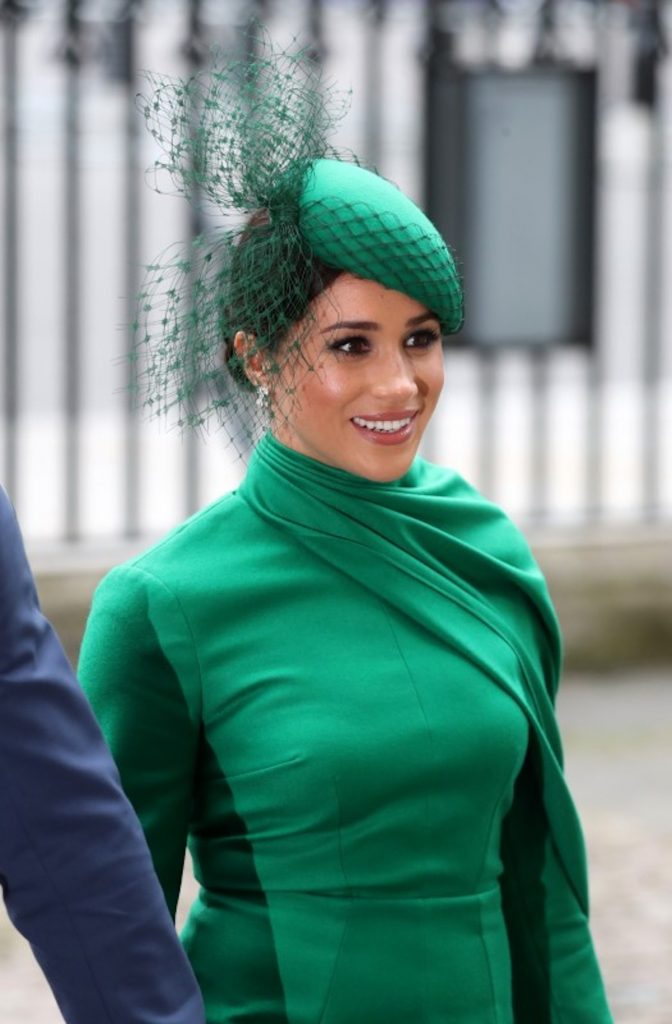
\includegraphics[scale=0.22]{meghan_markle.jpg}
            }
            \only<2>{
              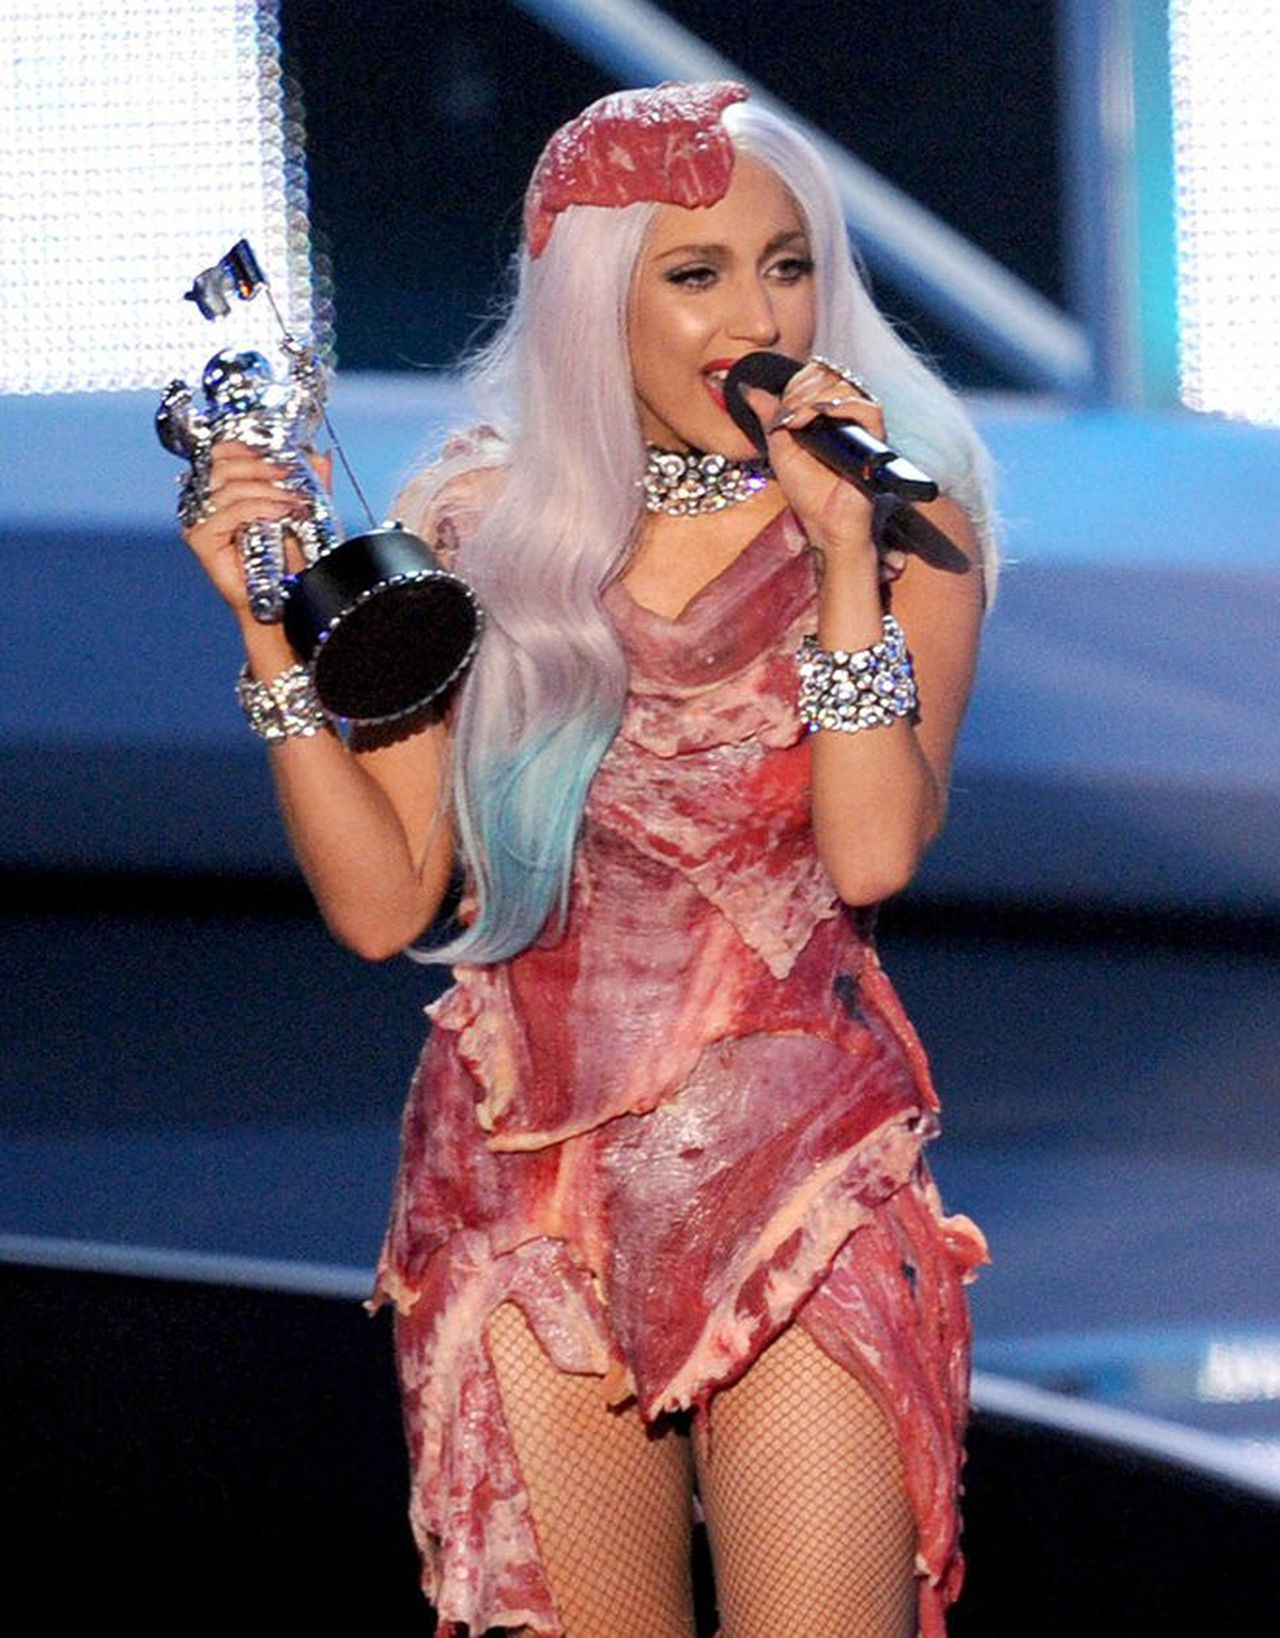
\includegraphics[scale=0.1]{lady_gaga.jpg}
            }
            \only<3>{
              
\includegraphics[scale=0.14]{oprah.jpg}
            }
            \only<4>{
              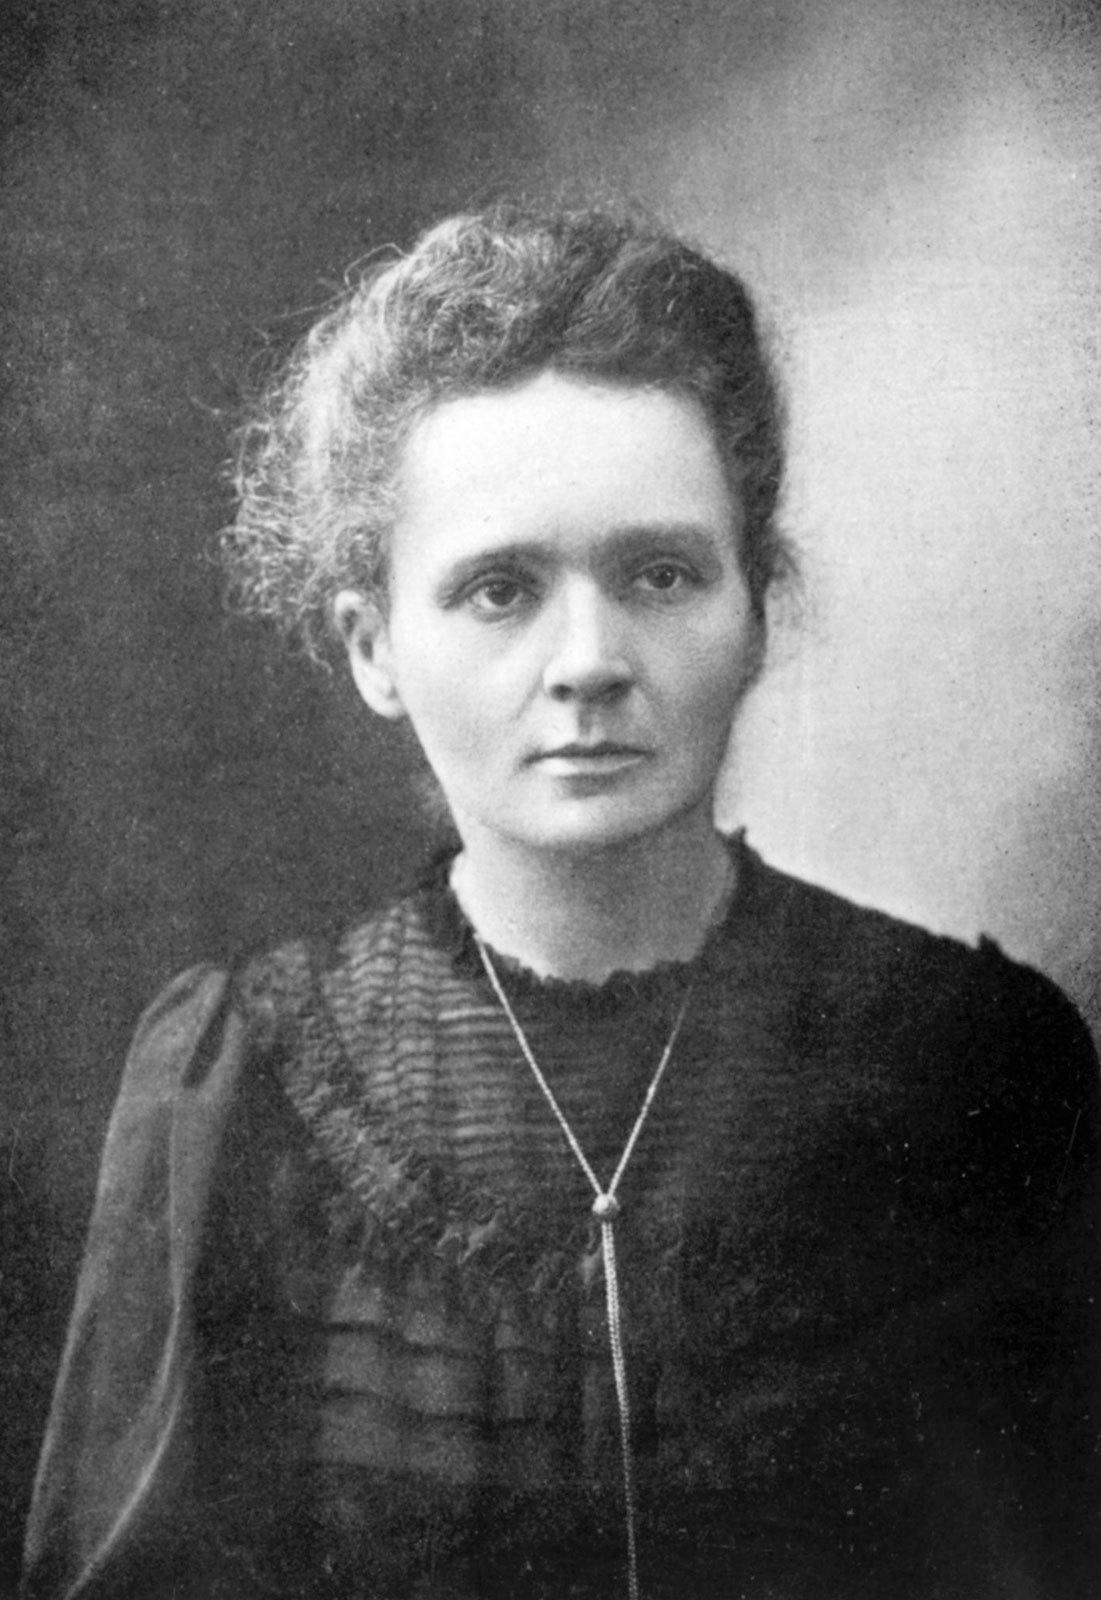
\includegraphics[scale=0.1]{marie_curie.jpg}
            }
            \only<5>{
              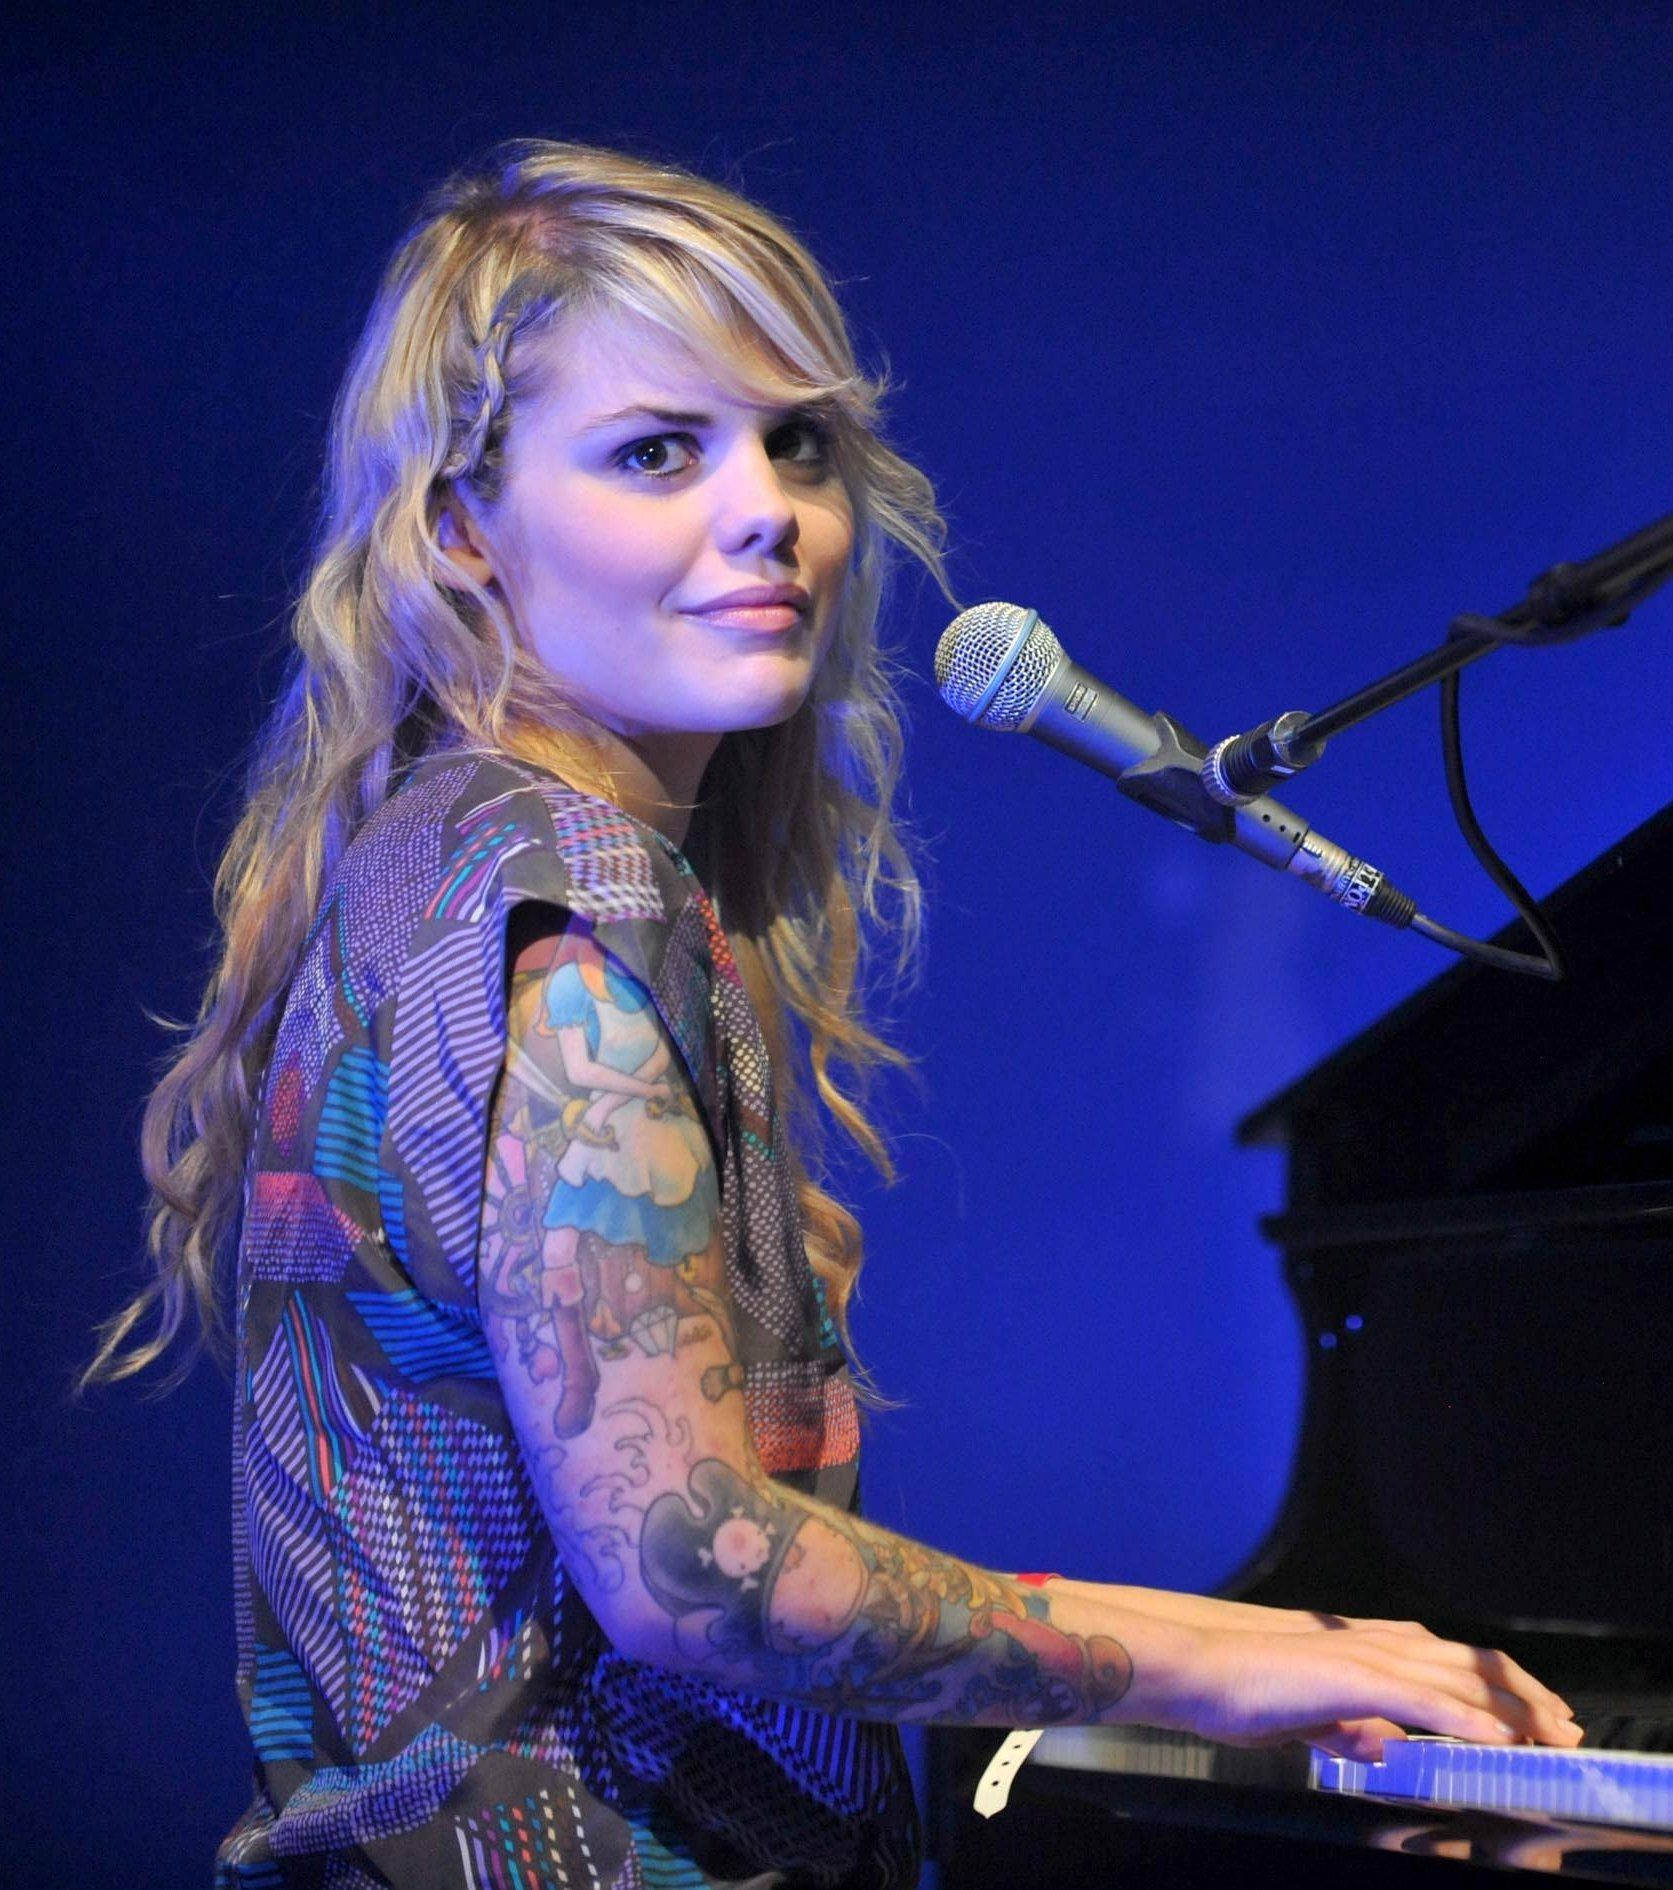
\includegraphics[scale=0.4]{coeur_de_pirate.jpg}
            }
          \end{center}
        \end{minipage}
    \end{columns}
  \end{frame}

  \begin{frame}{Une femme connue}
    En groupes de 3 ou 4, décrivez des femmes connues chacun à son tour, et faites deviner leurs identités à vos camarades. Décrivez non seulement leurs traits physiques mais leurs personnalités et activités. \\
    \tinygloss{In groups of 3 or 4, take turns describing well-known women, and have your groupmates guess at her identity.
    Describe not just their physical features but their personalities and activities.}
    \begin{columns}
      \column{0.5\textwidth}
        \begin{description}
          \item[E1:] Elle est sérieuse et drôle.
          \item[] \tinygloss{She's serious and funny.}
          \item[E2:] Est-ce que c'est la reine Elizabeth?
          \item[] \tinygloss{Is it Queen Elizabeth?}
          \item[E1:] Non! Ce n'est pas elle!
          \item[] \tinygloss{No! It's not her!}
        \end{description}
      \column{0.5\textwidth}
        \begin{center}
          
\includegraphics[scale=0.1]{projecteurs.jpg}
        \end{center}
    \end{columns}
  \end{frame}

  \begin{frame}{Les mots interrogatifs}
    Remplaçons la phrase en \emph{italique} avec le mot interrogatif le plus logique. \\
    \tinygloss{Let's replace the phrase in \emph{italics} with the most logical question word.}
    \begin{columns}[t]
      \column{0.5\textwidth}
        \begin{enumerate}
          \item Nous travaillons \emph{dans la salle de classe}.
          \item<2->[$\to$] \emph{Où} est-ce que nous travaillons?
          \item Il y a un examen \emph{mardi}.
          \item<3->[$\to$] \emph{Quand} est-ce qu'il y a un examen?
          \item Elle a \emph{deux} sœurs.
          \item<4->[$\to$] \emph{Combien de} sœurs est-ce qu'elle a?
        \end{enumerate}
      \column{0.5\textwidth}
        \begin{enumerate}
          \setcounter{enumi}{3}
          \item Yannick est absent \emph{parce qu'il est malade}.
          \item<5->[$\to$] \emph{Pourquoi} est-ce que Yannick est absent?
          \item \emph{Jacky} est généreuse.
          \item<6->[$\to$] \emph{Qui} est généreuse?
          \item Elle s'appelle \emph{Chloé Dupont}.
          \item<7->[$\to$] \emph{Comment} est-ce qu'elle s'appelle?
        \end{enumerate}
    \end{columns}
  \end{frame}

  \begin{frame}{Entrevue}
    Avec un/e camarade de classe avec qui tu n'as pas encore parlé, faites des entrevues en posant des questions aux sujets suivants.  \\
    \tinygloss{With a classmate that you haven't yet spoken to, interview each other by asking questions about the following subjects.}
    \begin{columns}
      \column{0.4\textwidth}
        \begin{enumerate}
          \item les amis
          \item la musique
          \item le sport
          \item les animaux
        \end{enumerate}
      \column{0.6\textwidth}
        \begin{center}
          
\includegraphics[scale=0.3]{entretien.png}
        \end{center}
    \end{columns}
  \end{frame}

  \begin{frame}{}
    \begin{center}
      \Large Questions?
    \end{center}
  \end{frame}
\end{document}
